\documentclass[final]{beamer}

% ====================
% Packages
% ====================

\usepackage[T1]{fontenc}
\usepackage{lmodern}
\usepackage[size=custom,width=120,height=72,scale=1.0]{beamerposter}
\usetheme{gemini}
\usecolortheme{uchicago}
\usepackage{graphicx}
\usepackage{booktabs}
\usepackage{doi}
\usepackage[numbers]{natbib}
\usepackage[patch=none]{microtype}
\usepackage{tikz}
\usepackage{pgfplots}
\pgfplotsset{compat=1.18}
\usepackage{anyfontsize}
\usepackage{subfig}

\pdfstringdefDisableCommands{%
\def\translate#1{#1}%
}

% ====================
% Lengths
% ====================

% If you have N columns, choose \sepwidth and \colwidth such that
% (N+1)*\sepwidth + N*\colwidth = \paperwidth
\newlength{\sepwidth}
\newlength{\colwidth}
\setlength{\sepwidth}{0.025\paperwidth}
\setlength{\colwidth}{0.3\paperwidth}

\newcommand{\separatorcolumn}{\begin{column}{\sepwidth}\end{column}}

% ====================
% Title
% ====================

\title{Elucidation of the mechanism of a Morita-Baylis-Hillman type reaction catalyzed by engineered enzymes using transition path sampling}

\author{Sree Ganesh Balasubramani \inst{1} \and Steven Schwartz \inst{1} }

\institute[shortinst]{\inst{1} Department of Chemistry and Biochemistry, The University of Arizona}

% ====================
% Footer (optional)
% ====================

\footercontent{
  \href{https://www.example.com}{https://sreeganb.github.io} \hfill
  %ABC Conference 2025, New York --- XYZ-1234 
  \hfill
  \href{mailto:sreegb@arizona.edu}{sreegb@arizona.edu}}
% (can be left out to remove footer)

% ====================
% Logo (optional)
% ====================

% use this to include logos on the left and/or right side of the header:
% \logoright{\includegraphics[height=7cm]{logo1.pdf}}
% \logoleft{\includegraphics[height=7cm]{logo2.pdf}}

% ====================
% Body
% ====================

\begin{document}
\addtobeamertemplate{headline}{}
{
    \begin{tikzpicture}[remember picture,overlay]
      \node [anchor=north west, inner sep=3cm] at ([xshift=0.0cm,yshift=-2.4cm]current page.north west)
      {
\includegraphics[height=5.0cm]{logos/ua_stack_rgb_4.eps}}; % also try shield-white.eps
      %\node [anchor=north east, inner sep=3cm] at ([xshift=0.0cm,yshift=2.5cm]current page.north east)
      %{\includegraphics[height=8.0cm]{logos/cs-logo-white.png}};
    \end{tikzpicture}
}

\begin{frame}[t]
\begin{columns}[t]
\separatorcolumn

\begin{column}{\colwidth}

\begin{block}{Directed evolution and the design of enzymes}
A series of engineered enzymes to perform the complex Morita-Bayliss-Hilmann reaction \cite{Crawshaw22NatChem14p313} 
    \begin{itemize}
     % \item Is it possible to design enzymes that perform complicated reactions such as this easily?
      \item Elucidate the mechanism and transition state of the double proton transfer reaction 
      %\item Find the transition state and propose mutations that improve the catalytic efficiency
      \item Understand the importance of quantum mechanical tunneling in the proton transfer
    \end{itemize}
 
  \end{block}

\begin{block}{Molecular dynamics simulations}
\begin{itemize}
\item Atomistic simulations to understand chemical reactions catalyzed by enzymes.
\item Partition the enzyme into regions treated using classical molecular mechanics (MM)
and quantum mechanics (QM)
\item A density functional approximation called SCCDFTB is the choice for the QM method
\end{itemize}

\begin{figure}
\subfloat[]{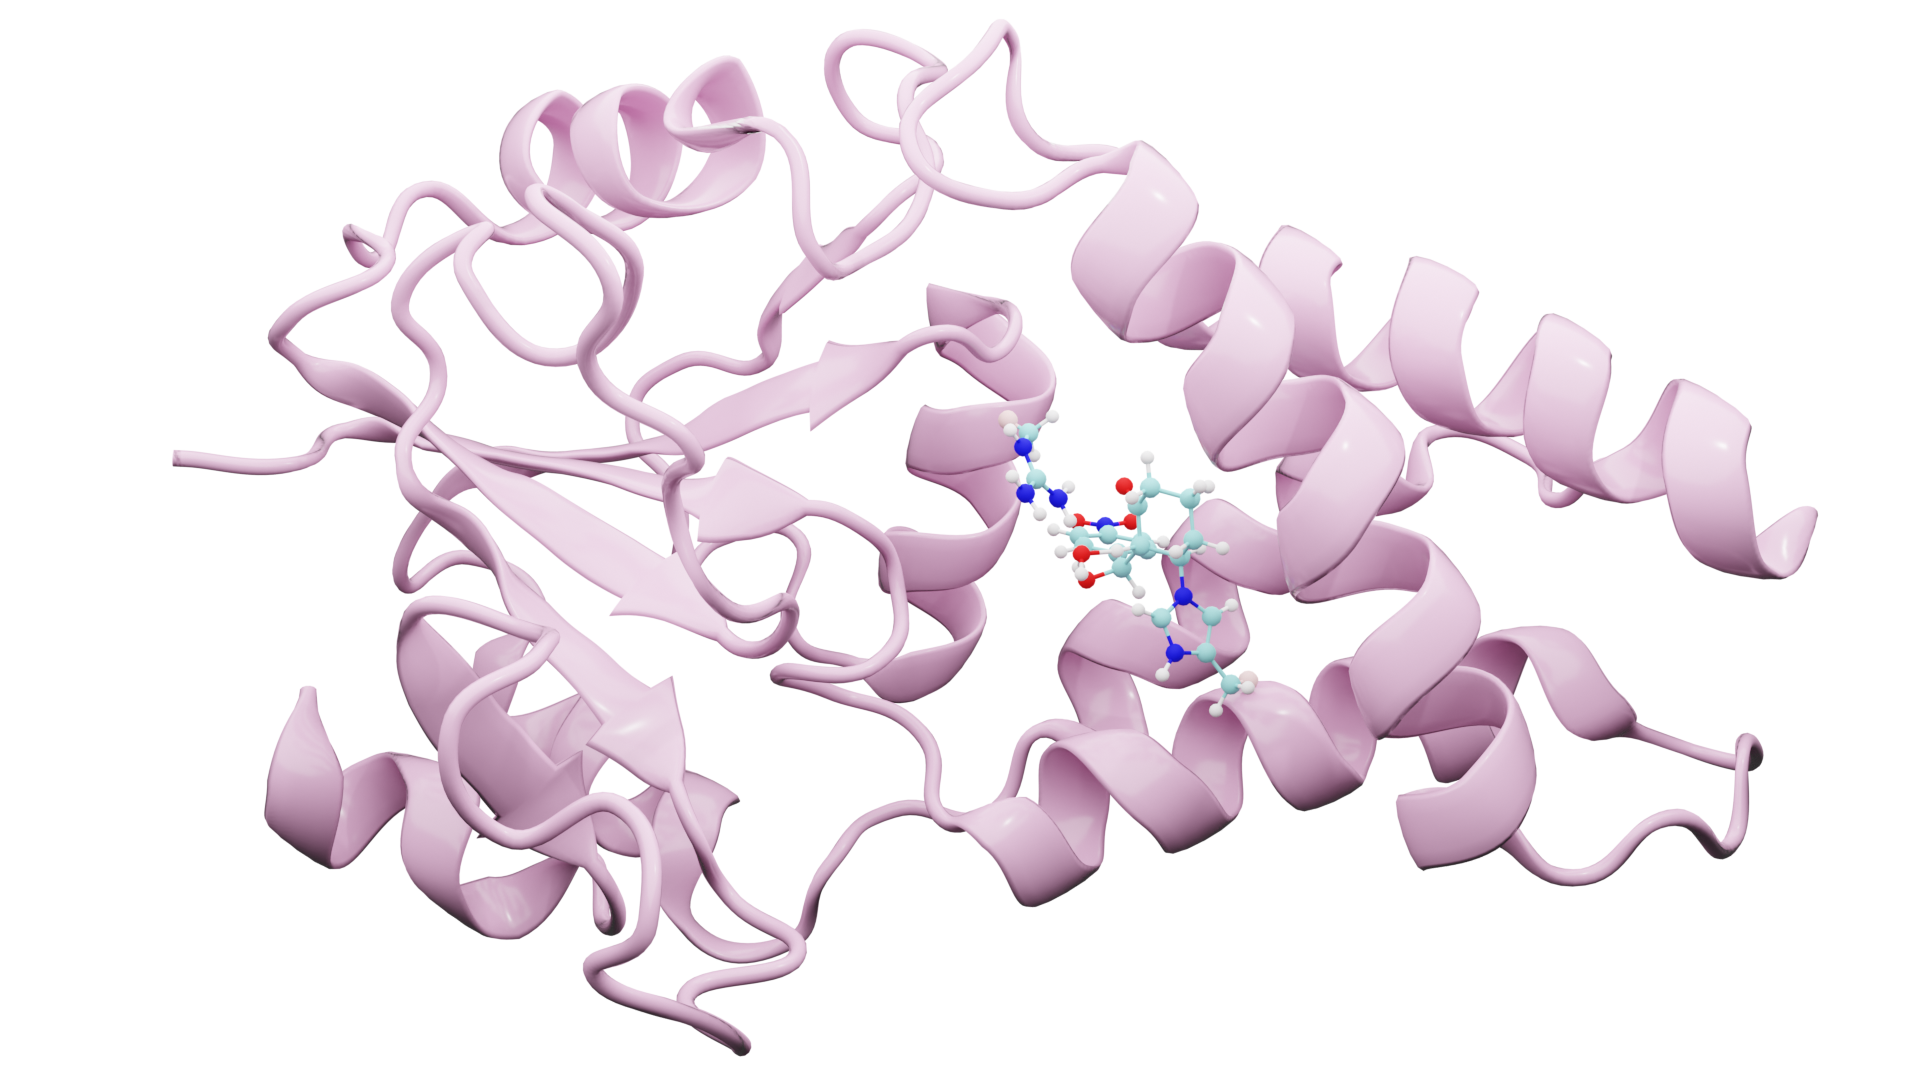
\includegraphics[width=0.55\colwidth]{figures/mbhase.png}}
\quad
\subfloat[]{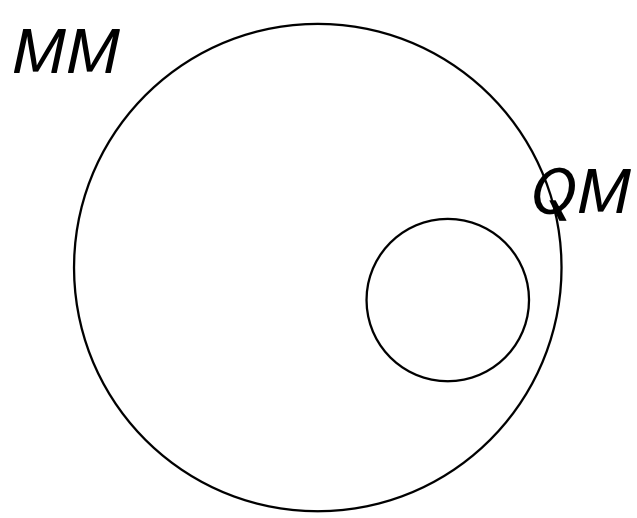
\includegraphics[width=0.38\colwidth]{figures/qmmm.png}}
\end{figure}
\end{block}

  \begin{block}{Introduction to TPS}
\begin{itemize}
    \item Enhanced sampling technique
    \item Monte-Carlo type method in the trajecotry space
    \item Elucidate the transition state, reaction coordinates, thermodynamic and kinetic parameters
    %\item Shooting and shifting algorithm
\end{itemize}
\begin{figure}%
\centering
\subfloat[Trajectories in phase space]{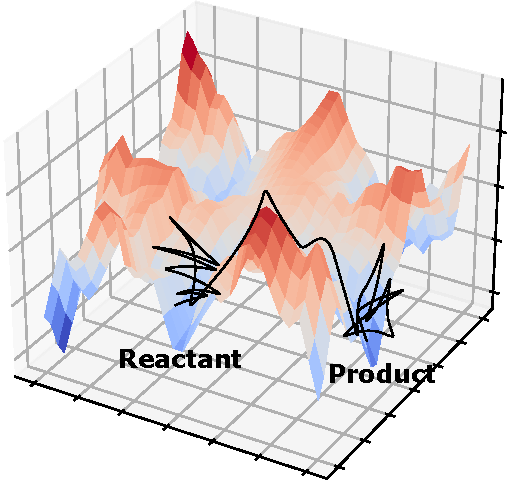
\includegraphics[width=0.45\colwidth]{figures/pot-surf.pdf}}%
\qquad
\subfloat[Shooting algorithm]{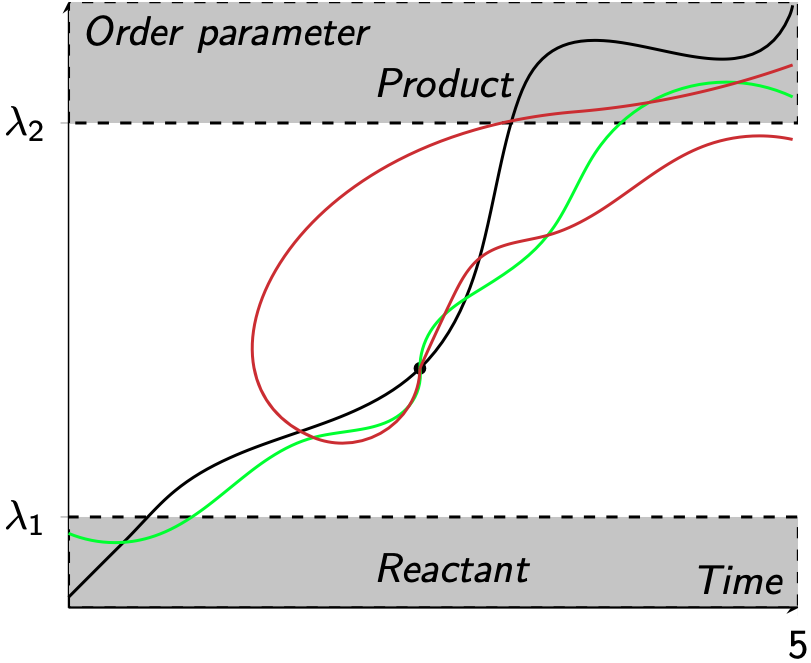
\includegraphics[width=0.45\colwidth]{figures/tps-desc.png}}
%\caption{Lets see}%
\label{fig:tps-desc}%
\end{figure}

  \end{block}

\end{column}

\separatorcolumn

\begin{column}{\colwidth}

  \begin{block}{Reactant and product states}
  \begin{figure}%
\centering
\subfloat[Reactant state]{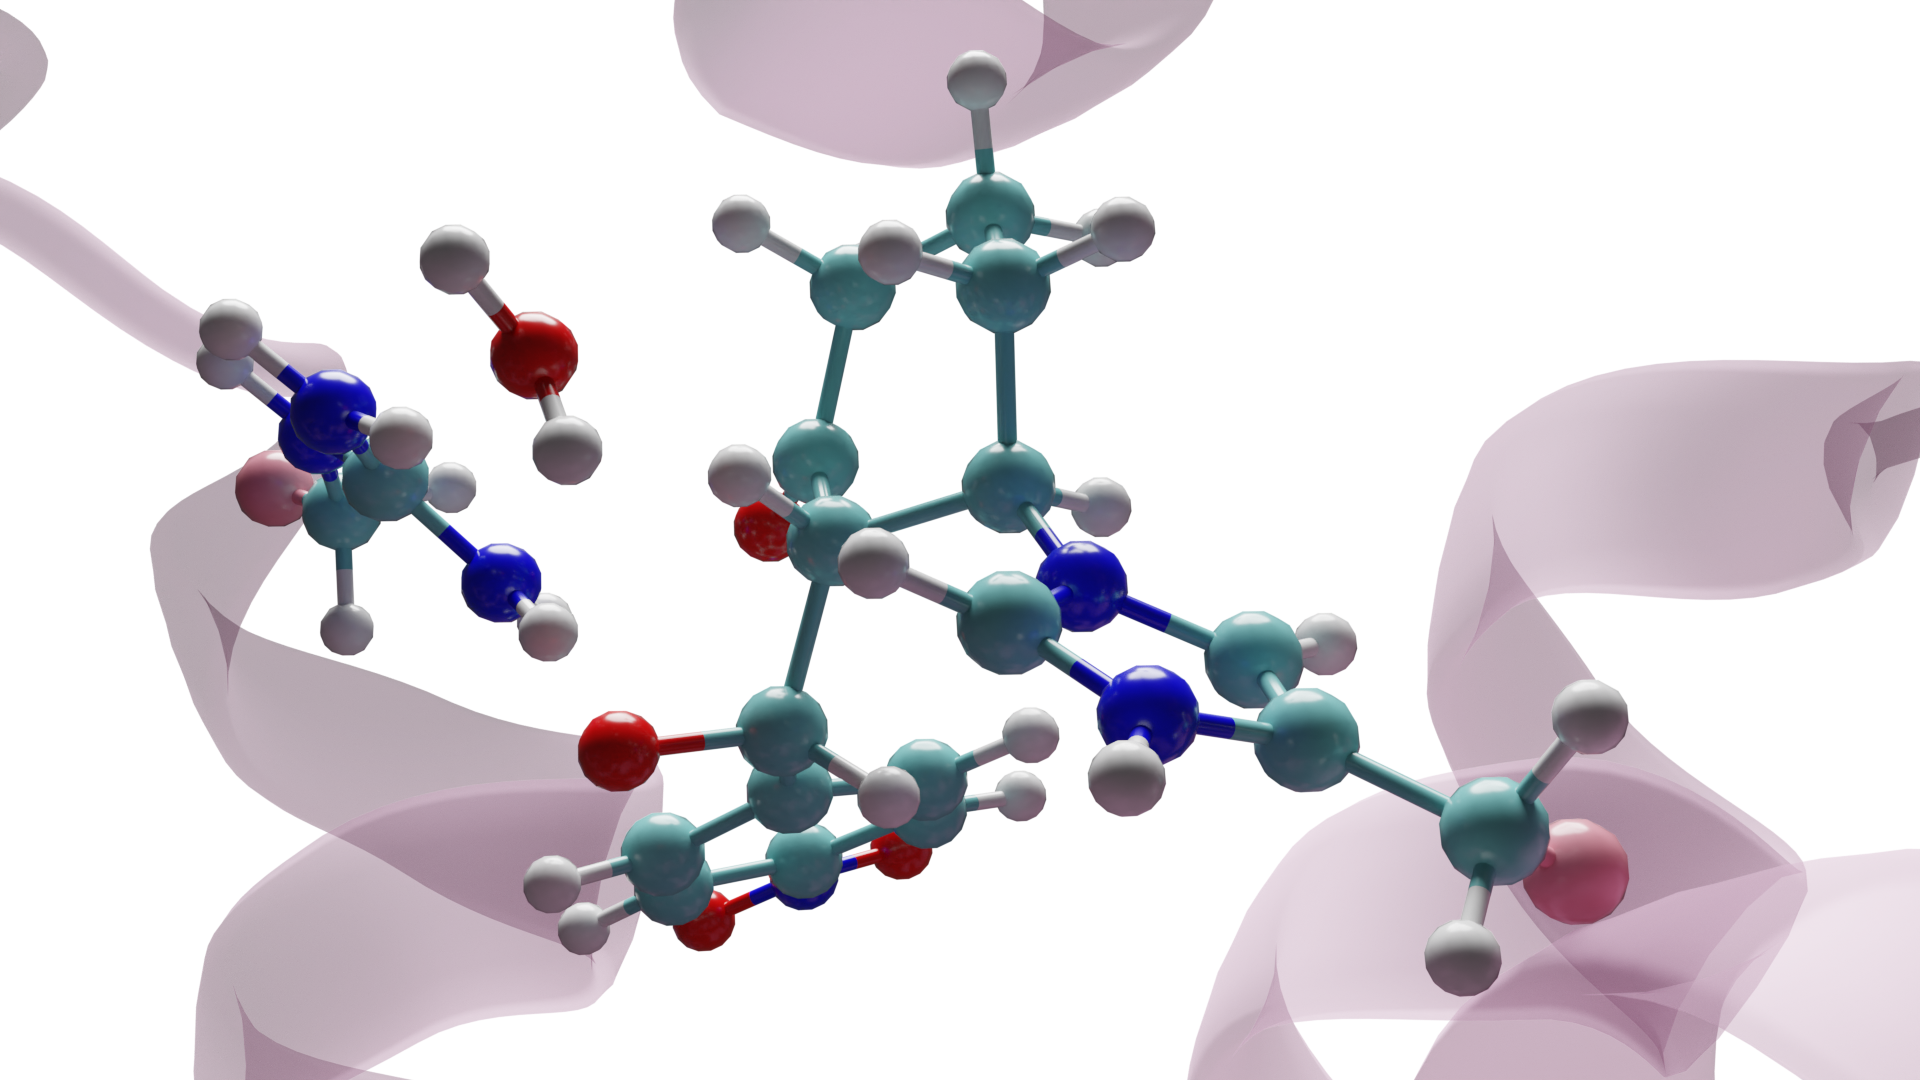
\includegraphics[width=0.45\colwidth]{figures/reac-120.png}}%
\quad
\subfloat[Product state]{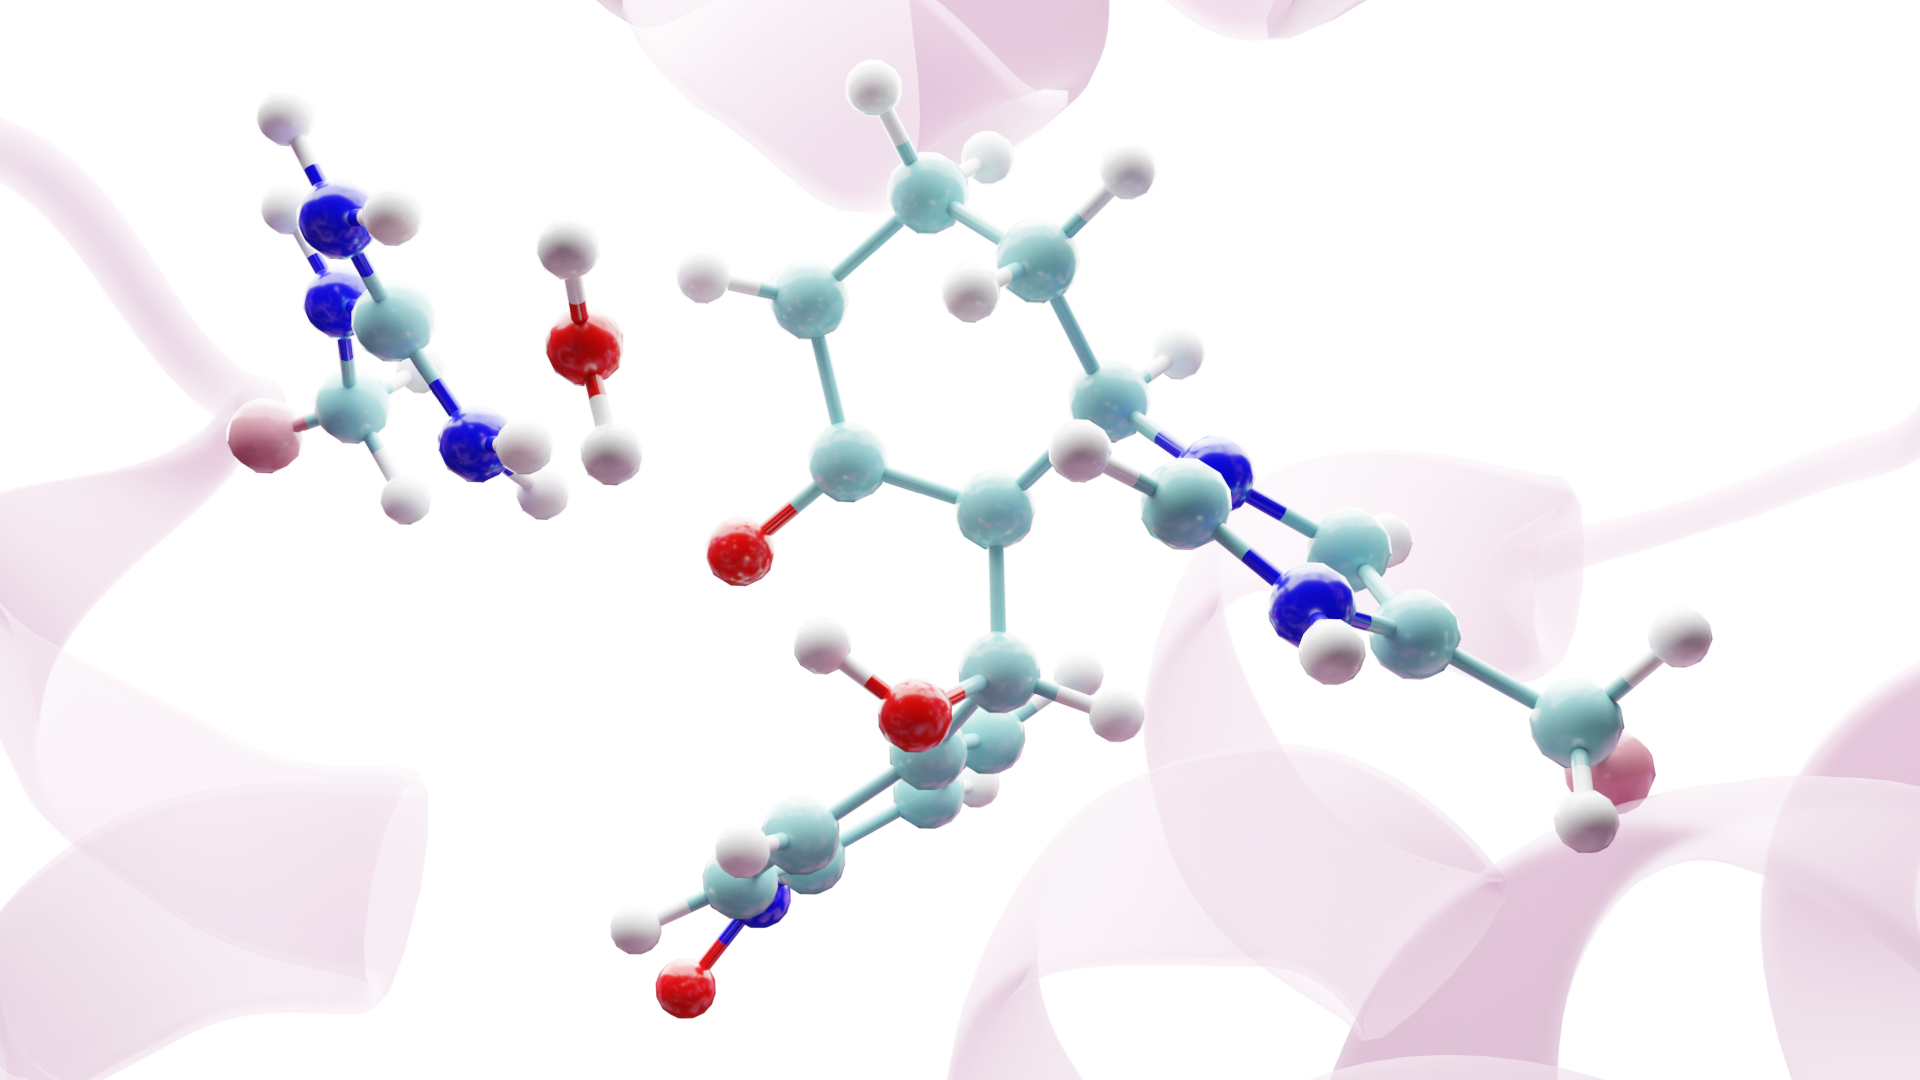
\includegraphics[width=0.45\colwidth]{figures/prod-120.png}}
%\caption{Lets see}%
\label{fig:tps-states}%
\end{figure}
   
  \end{block}

  \begin{block}{Committor analysis and transition state}
  \begin{figure}
        \subfloat[Committor]{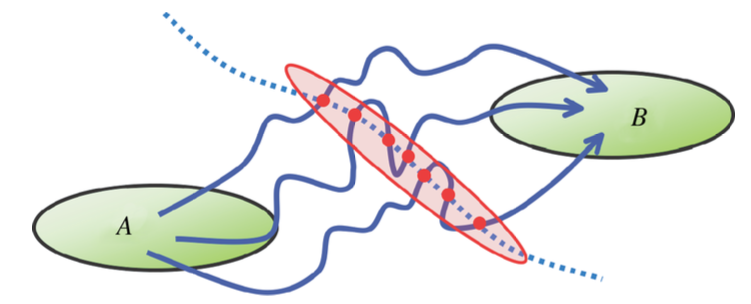
\includegraphics[width=0.4\colwidth]{figures/separatrix-full.png}}
        \qquad
        \subfloat[Transition State]{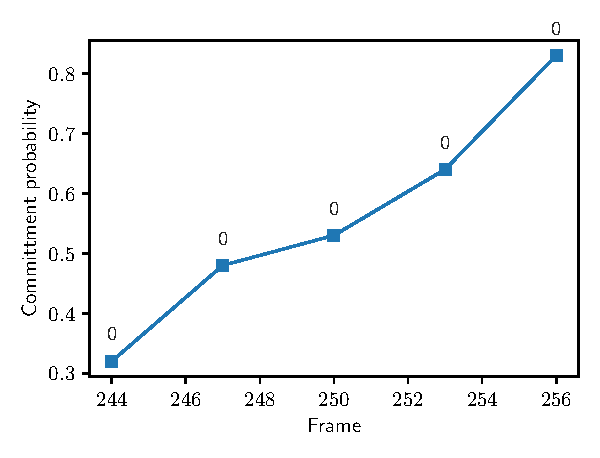
\includegraphics[width=0.5\colwidth]{figures/dist120.pdf}}
        %\caption{The protein witht he substrates bound}
    \end{figure}

  \end{block}

  \begin{block}{Transition state structure of the MBHase enzyme}
\begin{figure}
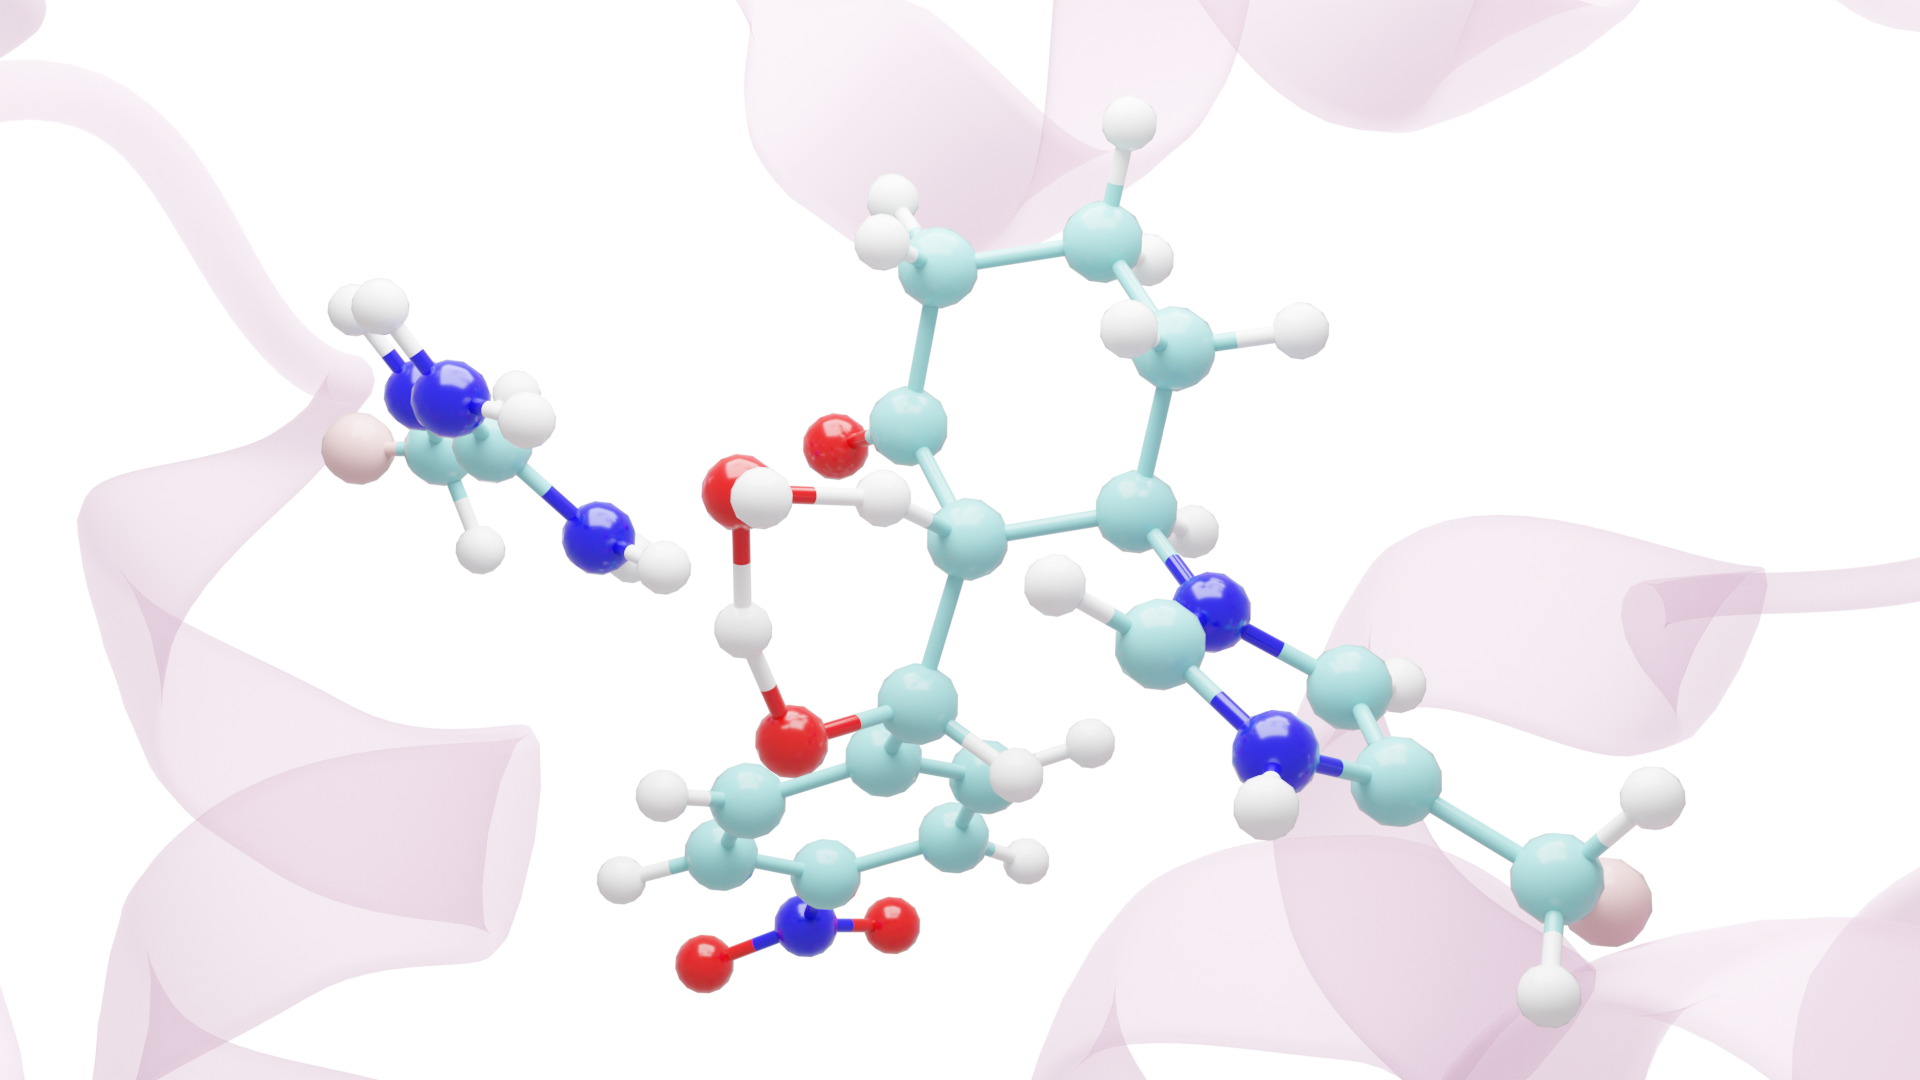
\includegraphics[width=0.6\colwidth]{figures/trans-120.png}
\end{figure}
  \end{block}

\end{column}

\separatorcolumn

\begin{column}{\colwidth}

  

  \begin{block}{Free energies from TPS}
    A method to calculate the free energies within TPS was recently applied to enzyme catalyzed reactions. \cite{Balasubramani22JPhysChemB126p5413}
    \begin{figure}
        \centering
        \subfloat[Modified shooting algorithm]{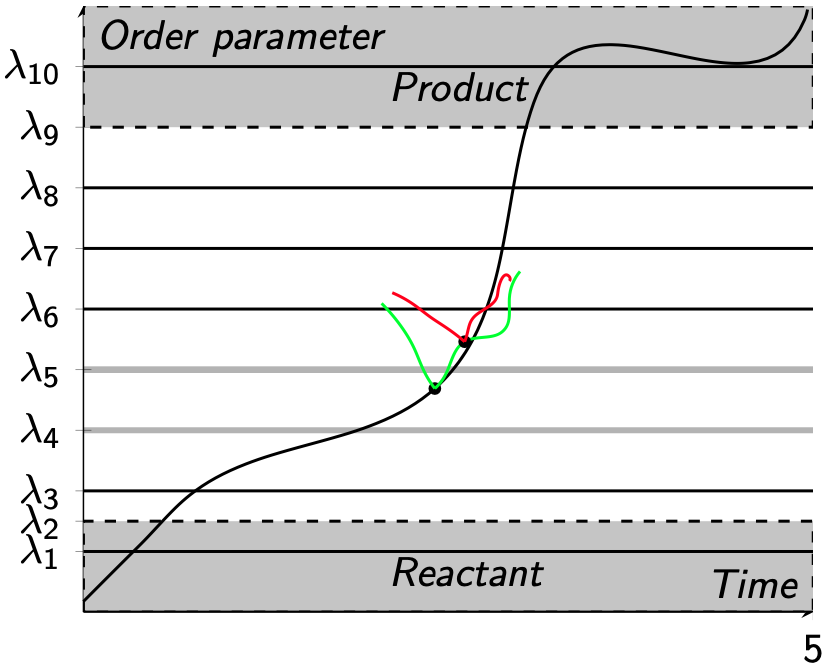
\includegraphics[width=0.4\colwidth]{figures/tps-free.png}}
        \quad
        \subfloat[Calculated Free energy for reaction catalyzed by the human MAT2A enzyme]{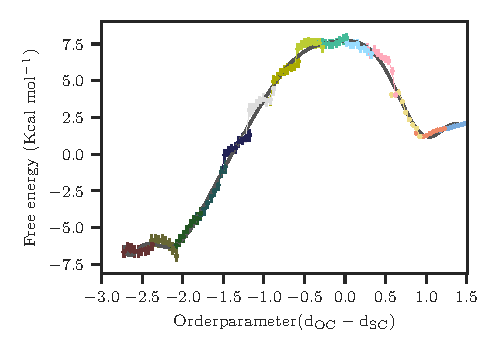
\includegraphics[width=0.5\colwidth]{figures/mat2a-fenergy.pdf}}
        %\caption{Modified shooting algorithm to calculate free energies}
    \end{figure}
    
  \end{block}
\begin{block}{Conclusions and future directions}
\begin{itemize}
    \item The transition state structure for the reaction catalyzed by an early 
    variant of the evolutionary process of the MBHase enzyme was obtained
    \item The transition state for the double proton transfer reaction proceeds through 
\end{itemize}
    
  \end{block}
  \begin{block}{References}

    \nocite{*}
    \footnotesize{\bibliographystyle{plainnat}\bibliography{poster}}

  \end{block}

\end{column}

\separatorcolumn
\end{columns}
\end{frame}

\end{document}
